% Asset ID: FAS1MatricesInvariantLinesTikZ-001
% Unit: FAS1
% Topic Code: FAS1-MAT
% Topic ID: FAS1MatricesInvariantLines
% Lesson File: FAS1_matrices_invariant_lines_lesson.md
% Related Lesson Section: # 9. Visual Asset Integration
% Source: CCEA FAS1-MAT specification boundary
% Purpose: Precise coordinate diagram for invariant lines under A = [[2,1],[3,0]]

\documentclass[tikz,border=8pt]{standalone}
\usepackage{amsmath}
\usepackage{xcolor}
\definecolor{Canvas}{HTML}{FAF9F6}
\definecolor{Ink}{HTML}{2C2C2E}
\definecolor{SoftLine}{HTML}{E5E5EA}
\definecolor{Gold}{HTML}{C5A059}
\definecolor{DeepGold}{HTML}{D4AF37}
\definecolor{Rose}{HTML}{FBEFEF}
\begin{document}
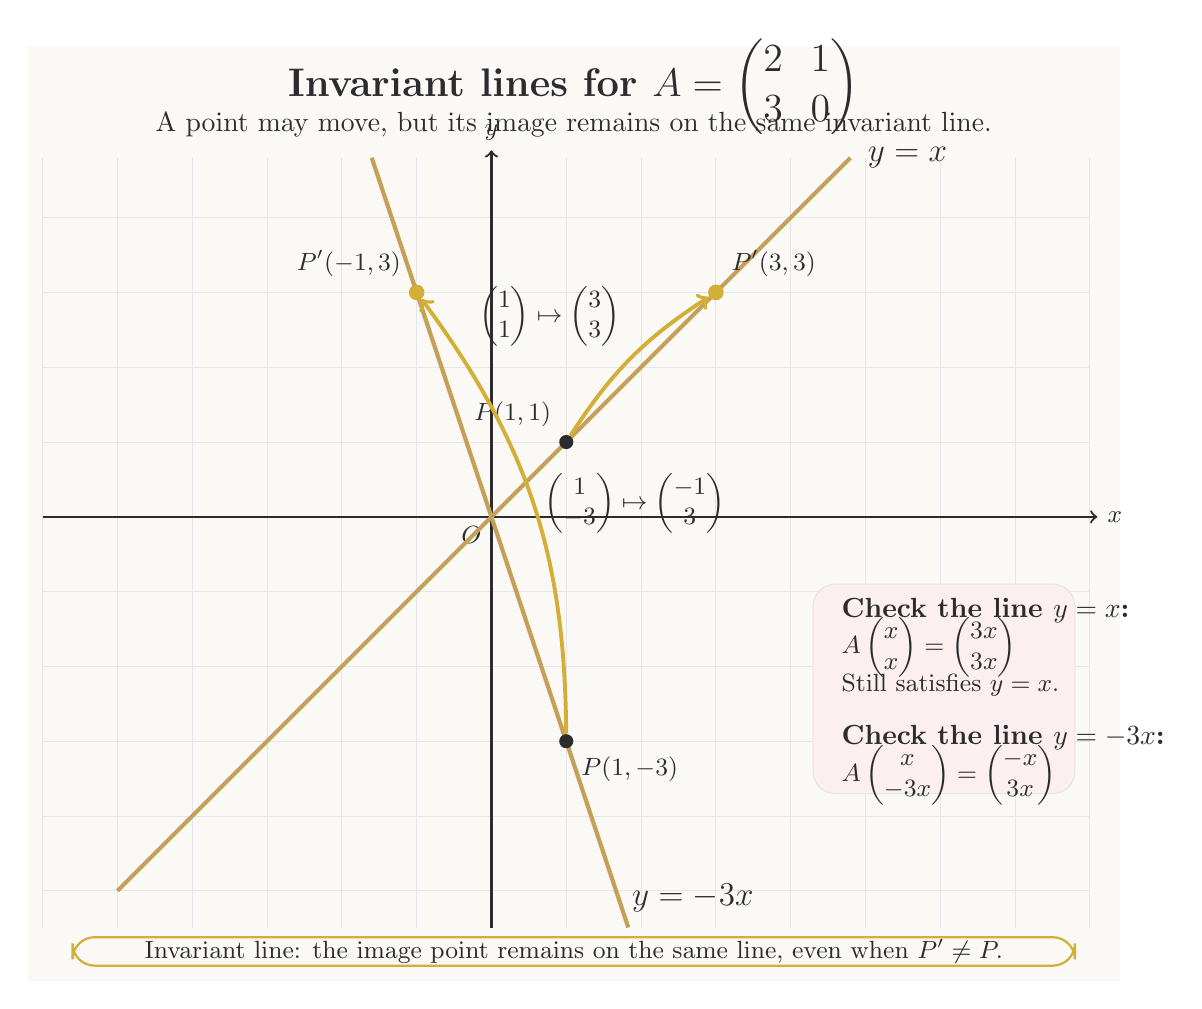
\begin{tikzpicture}[scale=0.95,every node/.style={font=\small,text=Ink},axis/.style={->,thick,draw=Ink},gridline/.style={draw=SoftLine,line width=0.35pt},invariant/.style={draw=Gold,line width=1.5pt},mover/.style={->,draw=DeepGold,line width=1.4pt},point/.style={circle,fill=Ink,inner sep=1.8pt},imagepoint/.style={circle,fill=DeepGold,inner sep=2pt}]
\fill[Canvas] (-6.2,-6.2) rectangle (8.4,6.3);
\node[font=\Large\bfseries] at (1.1,5.75) {Invariant lines for \(A=\begin{pmatrix}2&1\\3&0\end{pmatrix}\)};
\node[font=\normalsize] at (1.1,5.25) {A point may move, but its image remains on the same invariant line.};
\foreach \x in {-6,-5,...,8}{\draw[gridline] (\x,-5.5)--(\x,4.8);}
\foreach \y in {-5,-4,...,4}{\draw[gridline] (-6,\y)--(8,\y);}
\draw[axis] (-6,0)--(8.1,0) node[right]{\(x\)};
\draw[axis] (0,-5.5)--(0,4.9) node[above]{\(y\)};
\node[below left] at (0,0){\(O\)};
\draw[invariant] (-5,-5)--(4.8,4.8);
\node[anchor=west,font=\large] at (4.9,4.8){\(y=x\)};
\draw[invariant] (-1.6,4.8)--(1.83,-5.49);
\node[anchor=west,font=\large] at (1.75,-5.1){\(y=-3x\)};
\node[point,label=above left:{\(P(1,1)\)}] (P1) at (1,1) {};
\node[imagepoint,label=above right:{\(P'(3,3)\)}] (Q1) at (3,3) {};
\draw[mover,bend left=12] (P1) to node[midway,above left]{\(\begin{pmatrix}1\\1\end{pmatrix}\mapsto\begin{pmatrix}3\\3\end{pmatrix}\)} (Q1);
\node[point,label=below right:{\(P(1,-3)\)}] (P2) at (1,-3) {};
\node[imagepoint,label=above left:{\(P'(-1,3)\)}] (Q2) at (-1,3) {};
\draw[mover,bend right=18] (P2) to node[midway,right]{\(\begin{pmatrix}1\\-3\end{pmatrix}\mapsto\begin{pmatrix}-1\\3\end{pmatrix}\)} (Q2);
\filldraw[fill=Rose,draw=SoftLine,rounded corners=8pt] (4.3,-3.7) rectangle (7.8,-0.9);
\node[anchor=west,font=\bfseries] at (4.55,-1.25) {Check the line \(y=x\):};
\node[anchor=west] at (4.55,-1.75) {\(\displaystyle A\begin{pmatrix}x\\x\end{pmatrix}=\begin{pmatrix}3x\\3x\end{pmatrix}\)};
\node[anchor=west] at (4.55,-2.25) {Still satisfies \(y=x\).};
\node[anchor=west,font=\bfseries] at (4.55,-2.95) {Check the line \(y=-3x\):};
\node[anchor=west] at (4.55,-3.45) {\(\displaystyle A\begin{pmatrix}x\\-3x\end{pmatrix}=\begin{pmatrix}-x\\3x\end{pmatrix}\)};
\filldraw[fill=Canvas,draw=DeepGold,rounded corners=8pt,line width=0.8pt] (-5.6,-6.0) rectangle (7.8,-5.62);
\node at (1.1,-5.81) {\(\text{Invariant line: the image point remains on the same line, even when }P'\neq P.\)};
\end{tikzpicture}
\end{document}
